\chapter{Competition}

We compare the \emph{MM} and \emph{MMC} algorithms to \emph{Ratio} 
\cite{lowe2004sift} as well as \emph{Isomatch} \cite{das2008event} and 
\emph{Spectral} \cite{leordeanu2005spectral}.  \emph{Isomatch} and 
\emph{Spectral} uses geometric constraints, whereas \emph{Ratio} does 
not.

\begin{algorithm}
\caption{Ratio Match (\emph{Ratio})}
\label{alg-ratio}
%{\fontsize{10}{10}\selectfont
\begin{algorithmic}
\Require $im_1$ : image, $im_2$ : image, $t \in \mathbb{R}$
\State $matches\gets \varnothing$
\State $features_1 \gets getFeatures(im_1)$
\State $features_2 \gets getFeatures(im_2)$
\ForAll{$f_i \in features_1$}
    \State $f_m,f_n \gets get2NNs(f_i, features_2)$
	\State $ratio \gets similarity(f_i, f_n) / similarity(f_i, f_m)$
	\If{$ratio < t$}
        \State $matches \gets \left(f_i, f_m\right)$
	\EndIf
\EndFor
\Return $matches$
\end{algorithmic}
%}
\end{algorithm}

\emph{Ratio} (Algorithm~\ref{alg-ratio}) \cite{lowe2004sift} is the most 
straightforward of the three reference algorithms. Feature points are 
matched using K Nearest Neighbor and the similarity ratio between the 
best and second best match is then compared to a threshold to decide if 
the match is kept.

\begin{algorithm}
\caption{Isodata Match (\emph{Isomatch})}
\label{alg-isodata}
%{\fontsize{10}{10}\selectfont
\begin{algorithmic}
\Require $im_1$ : image, $im_2$ : image, $t \in \mathbb{R}$
\State $matches_{init}\gets \varnothing$
\State $matches_{final}\gets \varnothing$
\State $features_1 \gets getFeatures(im_1)$
\State $features_2 \gets getFeatures(im_2)$
\ForAll{$f_i \in features_1$}
    \State $f_m,f_n \gets get2NNs(f_i, features_2)$
    \State $matches_{init} \gets \left(f_i, f_m\right)$
\EndFor
\State $partitions_1 \gets isodata(getPositions(features_1))$
\State $partitions_2 \gets isodata(getPositions(features_2))$
\State $P_{corr} \gets getMatchMat(partitions_1, partitions_2, 
matches_{init})$
\ForAll{$(i,j) \in indices(P)$}
    \If{$\left(P_{i,j} > 5\right) \wedge \left(P_{i,j} / sum(P_{i}) > 
    0.5\right)$}
        \State $matches_{final} \gets getMatches(matches_{init}, 
        partitions_1, partitions_2, i, j)$
    \EndIf
\EndFor
\Return $matches_{final}$
\end{algorithmic}
%}
\end{algorithm}

\begin{figure}[htb]
	\centering
	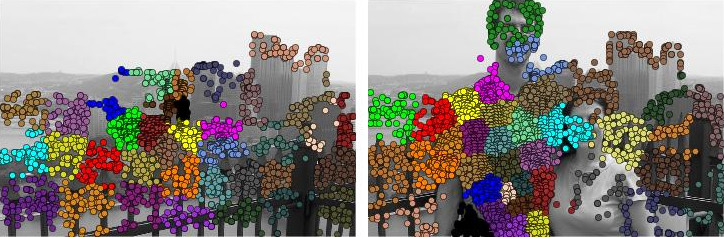
\includegraphics[width=\columnwidth]{images/isomatch_partitions}
	\caption{The result of partitioning feature points in two images.  
	Each dot represents a feature point and feature points grouped with 
the same color belong to the same partition.}
	\label{fig:isomatch_partitions}
\end{figure}

The \emph{Isomatch} algorithm (Algorithm~\ref{alg-isodata}) 
\cite{das2008event} is based on the idea that local feature points 
within a region in one image often matches to features within a 
corresponding region in the other image. To find these regions the 
algorithm uses the Isodata algorithm \cite{ball1965isodata} to perform 
unsupervised clustering on the feature points given their positions in 
the two images. The Isodata algorithm is similar to K-means with the 
addition that clusters are merged and split during the clustering 
process. In Figure~\ref{fig:isomatch_partitions} an example of a 
partitioning can be seen. The initial set of matches are filtered based 
on the resulting regions. A match is kept only if it at least half the 
matches of the same region of origin also belong to the same region in 
the other image.  $P_{corr}$ in Algorithm~\ref{alg-isodata} is a matrix 
where each row corresponds to a region in $im_1$, each column 
corresponds to a region in $im_2$ and $P_{i,j}$ is the amount of matches 
going from region $i$ to region $j$.

To threshold the \emph{Isomatch} algorithm we filter the results using 
the ratio between first and second best match as in \emph{Ratio}, since 
\emph{Isomatch} itself doesn't readily admit any thresholding parameter.  

\begin{algorithm}[h!]
\caption{Spectral Match (\emph{Spectral})}
\label{alg-spectral}
%{\fontsize{10}{10}\selectfont
\begin{algorithmic}
\Require $im_1$ : image, $im_2$ : image, $t \in \mathbb{R}$
\State $matches_{init}\gets \varnothing$
\State $matches_{final} \gets \varnothing$
\State $features_1 \gets getFeatures(im_1)$
\State $features_2 \gets getFeatures(im_2)$
\ForAll{$f_i \in features_1$}
	\State $f_m,f_n \gets get2NNs(f_i, features_2)$
	\State $matches_{init} \gets \left(f_i, f_m\right)$
\EndFor
\State $M \gets matrix(\left\vert matches_{init} \right\vert, \left\vert 
matches_{init} \right\vert)$
\ForAll{$m_i \in matches_{init}$}
	\ForAll{$m_j \in matches_{init}$}
		\If{$i = j$}
			\State $M \gets matchSimilarity(m_i)$
		\Else
			\State $M \gets affinity(m_i, m_j)$
		\EndIf
	\EndFor
\EndFor
\State $x^{*} \gets maximumEigenvector(M)$
\ForAll{$\left(m_i, x_i\right) \in \left(matches_{init}, x^{*}\right)$}
	\If{$x_i > t$}
		\State $matches_{final} \gets matchtes_{final} \cup m_i$
	\EndIf
\EndFor

\Return $matches_{final}$
\end{algorithmic}
%}
\end{algorithm}

The \emph{Spectral} algorithm (Algorithm~\ref{alg-spectral}) is a 
slightly modified version of the spectral matching algorithm proposed by
Leordeanu and Herbert \cite{leordeanu2005spectral}. It is based on the 
idea that the set of actual correspondences of feature points between 
two images should be pairwise consistent. That is, given two feature 
points that are geometrically close in one image, for most cases we 
would assume that the closest correspondences in another image would be 
similarly close. We want to pick out a set of matches $T \subset S$ 
where $S$ is the initial set of possible matches such that the matches 
in $T$ are as pairwise consistent as possible. If we let $x$ be a binary 
vector corresponding in length to the set of initial matches $S$, where 
$x_i = 1$ if $m_i \subset T$, then we can formulate a subset-score as:
\begin{equation*}
	S = \sum_{m_i, m_j \in T} M(m_i, m_j) = x^TMx
\end{equation*}
The solution $x^{*}$ that maximizes this equation is then $x^{*} = 
argmax(x^TMx)$. By relaxing the constraints on $x$ such that it can take
values in the range of $\left[0, 1\right]$ we can interpret $x_i$ as the
association of $m_i$ with the optimal subset of matches $T$. Because we 
only worry about the relative values of $x$ we can fix the norm of $x$ 
to $1$, in which case by Raleigh's ratio theorem, the $x^{*}$ that 
optimizes $x^TMx$ is the principal eigenvector of $M$.

Leordeanu and Herbert proposes a simple affinity function to map the 
pairwise distance of two matches. In a scene where no rotation and 
excessive affine transformation takes place, it can generally be assumed 
that the length and direction of the vector between
the two feature points constituting the first match corresponds to the 
length and direction of the vector between the two feature points 
constituting the second match. Given two matches $m_i = (f_{i,1}, 
f_{i,2})$ and $m_j = (f_{j,1},f_{j,2})$ where $f_{k,n}$ is the feature 
point of match $k$ in image $n$, we denote the euclidean distance 
between feature points $f_{i,n}$ and $f_{j,n}$ in image $n$ as 
$d_{i,j,n}$.  The affinity function assigning a score based on the 
pairwise distance is then defined as follows:
\begin{equation*}
	M(a,b) \begin{cases} 4.5 - \frac{\left(d_{i,j,1} - 
		d_{i,j,2}\right)^2}{2\sigma^2}, & \mbox{if } \left\vert 
				d_{i,j,1} - d_{i,j,2} \right\vert < 3\sigma \\ 0, & 
				\mbox{otherwise}
	\end{cases}
\end{equation*}
In the equation above $\sigma$ is a stabilizing parameter that controls 
the sensitivity of the score to deformations in the data. A larger 
$\sigma$ will allow for larger deformations. In the experiments it is 
fixed to 50. There are a number of occasions where the assumption that 
pairwise matches should have the same distance doesn't hold true.  A 
simple example would be matches between two images of the same scene 
where one image is rotated $180^{\circ}$.  However for a lot of 
applications like panorama stitching where we only see minor rotation 
and change of perspective the assumption is accurate.

In the implementation proposed by Leordeanu and Herbert 
\cite{leordeanu2005spectral} the last step of the algorithm greedily 
selects matches to ensure that matches are consistent, i.e.\ that two 
feature points in one image don't match with the same feature point in 
the other image. This is done by going through all the matches in the 
order of their associated $x^{*}$ score and for each match eliminating 
all matches in conflict with this match. This method ensure that as many
matches are kept as possible since only the conflicting matches are 
removed. However for cases where most feature points in one image will 
not have a correspondence in the other other image (e.g.\ cases of 
partial image overlap or object recognition) the greedy matching 
algorithm will keep finding matches even after the actual 
correspondences have already been found as long as they are consistent.

Since the testing is done on images with partial overlap, the final set 
of matches returned in Algorithm~\ref{alg-spectral} is the set of 
matches where the association of the match with the optimal subset of 
matches $T$ as measured by $x^{*}$ is above a certain threshold. For 
experiments the set of initial matches were given by the best match per 
feature point and the threshold was adjusted to allow for the best 50\% 
to be included in the set of final matches. A rate less than 50\% 
usually did not improve results, so to threshold the \emph{Spectral}
algorithm we filter the output using the ratio between first and second
best match as done in \emph{Ratio}.
